\documentclass[pdf, xcolor=table]{beamer}
\mode<presentation>{}
%%%%%%%%%% Temas %%%%






\setbeamercolor{section in toc}{fg=blue}
\setbeamercolor{subsection in toc}{fg=black}


\usepackage{adjustbox}
\usepackage{array}
\usepackage{stmaryrd}
\usepackage{graphicx}
\usecolortheme{beaver}
\usetheme{Pittsburgh}
\usepackage{appendixnumberbeamer}
%\usetheme[progressbar=frametitle]{metropolis}
\usepackage[backend = biber, style = abnt, extrayear, noslsn, repeatfirstfields]{biblatex}
\addbibresource{Bibliografia_Mestrado_FAPESP.bib}


\usepackage{ifthen} 
\newboolean{includethis} 
\setboolean{includethis}{false} 
\newcommand{\ifinclude}[1]{\ifthenelse{\boolean{includethis}}{#1}{}} 

\usepackage{ragged2e}
\justifying
\usepackage{parskip}
\setlength{\parskip}{\smallskipamount}


\usepackage[utf8]{inputenc}
\usepackage[brazil]{babel}
\usepackage[T1]{fontenc}
\usefonttheme{serif}
\usepackage{lipsum}
\usepackage{caption}
\setbeamercolor{block title}{bg=red!30,fg=black}
\usepackage{times}
\usepackage{tikz}
\usepackage{amsmath}
\usepackage{verbatim}
\usetikzlibrary{arrows,shapes}

\usepackage{float}
\usepackage{caption}

\newenvironment{variableblock}[3]{%
	\setbeamercolor{block body}{#2}
	\setbeamercolor{block title}{#3}
	\begin{block}{#1}}{\end{block}}

\author{Gabriel Petrini da Silveira \and RA 155468}
\title[Projeto]{Distribuição de renda, inclusão financeira e regime de metas para a inflação: compatibilidade ou conflito? Evidências para o caso brasileiro (2006-2016)}
\institute{Instituto de Economia - UNICAMP}
\date{2018}



\usepackage{xcolor}
\setbeamercolor{alerted text}{fg=blue}

\usepackage{color}
\definecolor{gray}{gray}{0.3}
\definecolor{darkgreen}{rgb}{0,0.55,0}
\definecolor{purple}{rgb}{0.5,0,1}
\setbeamercovered{transparent}

\usepackage{multirow}
\beamertemplatenavigationsymbolsempty


\usepackage{eso-pic}
\usepackage{ragged2e}
\usepackage{framed} 
\makeindex
%\setbeamertemplate{headline}{}
\usepackage{ulem}


\usepackage{tikz}
\usetikzlibrary{arrows,shapes,positioning,shadows,trees}

\usepackage[bottom]{footmisc}



\usepackage{arydshln}



\usetikzlibrary{arrows.meta,chains}

\usetikzlibrary{matrix}
\usepackage{multicol}
\usepackage{adjustbox}
\usepackage{graphicx}

\usepackage{arydshln}
\setbeamercolor{alerted text}{fg=red}

\hypersetup{colorlinks=true,citecolor=gray}

\newcommand*{\info}[4][16.3]{%
  \node [ annotation, #3, scale=0.65, text width = #1em,
          inner sep = 2mm ] at (#2) {%
  \list{$\bullet$}{\topsep=0pt\itemsep=0pt\parsep=0pt
    \parskip=0pt\labelwidth=8pt\leftmargin=8pt
    \itemindent=0pt\labelsep=2pt}%
    #4
  \endlist
  };
}

\def\firstcircle{(90:1.75cm) circle (2.5cm)}
  \def\secondcircle{(210:1.75cm) circle (2.5cm)}
  \def\thirdcircle{(330:1.75cm) circle (2.5cm)}

\begin{document}









\begin{frame}
\titlepage
\end{frame}

\begin{frame}{Resumo do período}

    O período a ser analisado pode ser caracterizado como \alert{crescimento econômico com inclusão social}:
    \begin{itemize}
        \item Crescimento com inflação (relativa) baixa
        \item \textit{Boom} de \textit{commodities}
        \item Crescimento da demanda externa
        \item Política de salário mínimo e crescimento do emprego
        \item Melhora (relativa) da desigualdade social
        \item \textit{Boom} de crédito
    \end{itemize}
\textbf{OBS:} Rolim (2017, rascunho) não foi incluído na bibliografia
\end{frame}



\begin{frame}{Diminuição da desigualdade}
    \begin{figure}[H]
    \caption{Desigualdade e distribuição de renda}
    \label{fig}
	\usetikzlibrary{arrows.meta,chains}
	\begin{tikzpicture}[
	> = latex',
	start chain = 1 going right,
	node distance=7mm,
	block/.style={shape=rectangle, draw,
		inner sep=1mm, align=center,
		minimum height=7mm, on chain}]     %Para que servem esses comandos?
	%placing the blocks
	\node[block] (n1) {$\Uparrow \Uparrow$ Desigualdade};
	\node[block, fill = gray!30] (n2) {Distribuição\\ de renda};
	\node[block] (n3) {$\Downarrow \Uparrow$ Desigualdade};
	

	
	\draw[->] (n1.east) --  + (0,0mm) -> (n2.west);
	\draw[->] (n2.east) --  + (0,0mm) -> (n3.west);
	\end{tikzpicture}

\end{figure}
A ideia da Figura \ref{fig} é mostrar que a distribuição de renda foi o meio de redução da desigualdade
\end{frame}


\begin{frame}{Distribuição de renda}
\framesubtitle{Participação na renda domiciliar (percentis selecionados)}
\begin{figure}[htb]
    \centering
    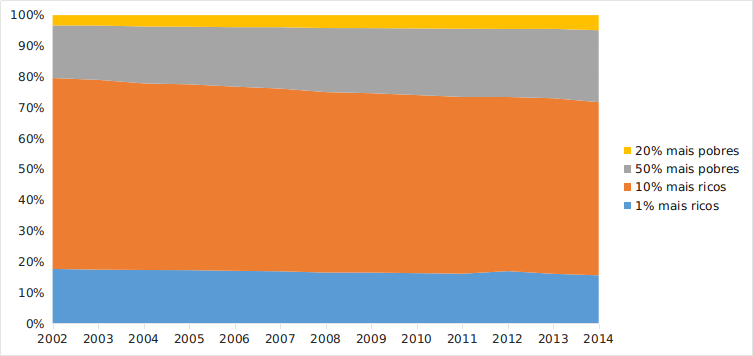
\includegraphics[width = 1.1\textwidth]{Part_Renda_Dom.png}
\end{figure}
    
\end{frame}

%\begin{frame}{Participação na renda disponível em percentis (2006-2015)}
 %   \begin{figure}
  %  \centering
   % \label{plot_Desigualdade}
    %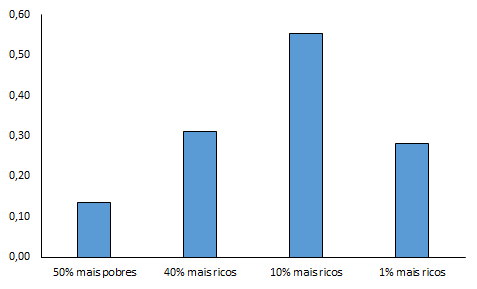
\includegraphics[width=0.8\paperwidth,height=0.8\paperheight]{Plot_Desigualdade.png}
%\end{figure}
%\end{frame}


\begin{frame}{Desigualdade}
\framesubtitle{Índice de Theil e Gini}

    \begin{figure}
    \centering
    \label{plot_Theil}
    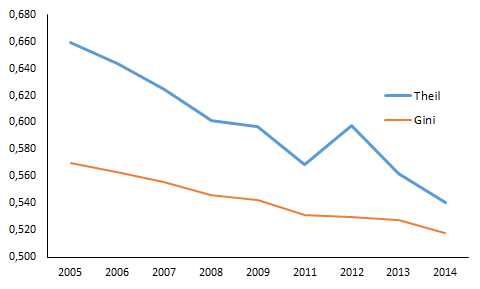
\includegraphics[width=0.8\paperwidth,height=0.8\paperheight]{Plot_Theil_Gini.png}
\end{figure}
\end{frame}


\begin{frame}{Um breve retrato do período}
\framesubtitle{Razão entre a renda dos 10\% mais ricos e a renda dos 40\% mais pobres}
\begin{figure}
    \centering
    \label{plot_Percentil}
    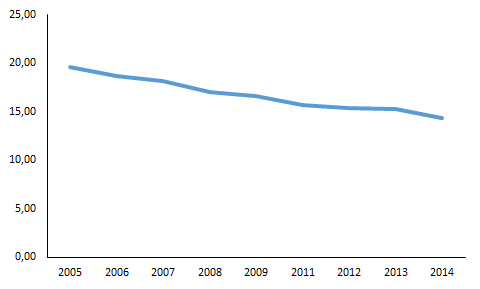
\includegraphics[width=0.8\paperwidth,height=0.8\paperheight]{Plot_Percentil_Rel.png}
\end{figure}
\end{frame}


\begin{frame}{Determinantes da redistribuição de renda (2006-2016)}
Analisando agora os mecanismos de distribuição da renda em favor dos salários. Os principais instrumentos foram:
    \begin{itemize}
        \item Aumentos reais do salários mínimo
        \item Políticas de transferência de renda
        \item \alert{Inclusão financeira}
    \end{itemize}
\vspace{1cm}

\begin{block}{Hipótese}    
Tais medidas ficaram restritas à esfera da conjuntura, ou seja, não implicaram em uma mudança \textbf{estrutural}
\end{block}
\end{frame}

\begin{frame}{Inclusão financeira}
Na literatura, a inclusão financeira é vista como aumento da relação bancária entre os adultos. Desse conceito desdobram algum temas correlatos:
\begin{itemize}
	\item Aprimoramento institucional
	\item Microcrédito e cooperativas de crédito
	\item Desburocratização
\end{itemize}
    
\end{frame}

\begin{frame}{Percentual de adultos com relacionamento bancário}
\begin{figure}
    \centering
    \label{plot1}
    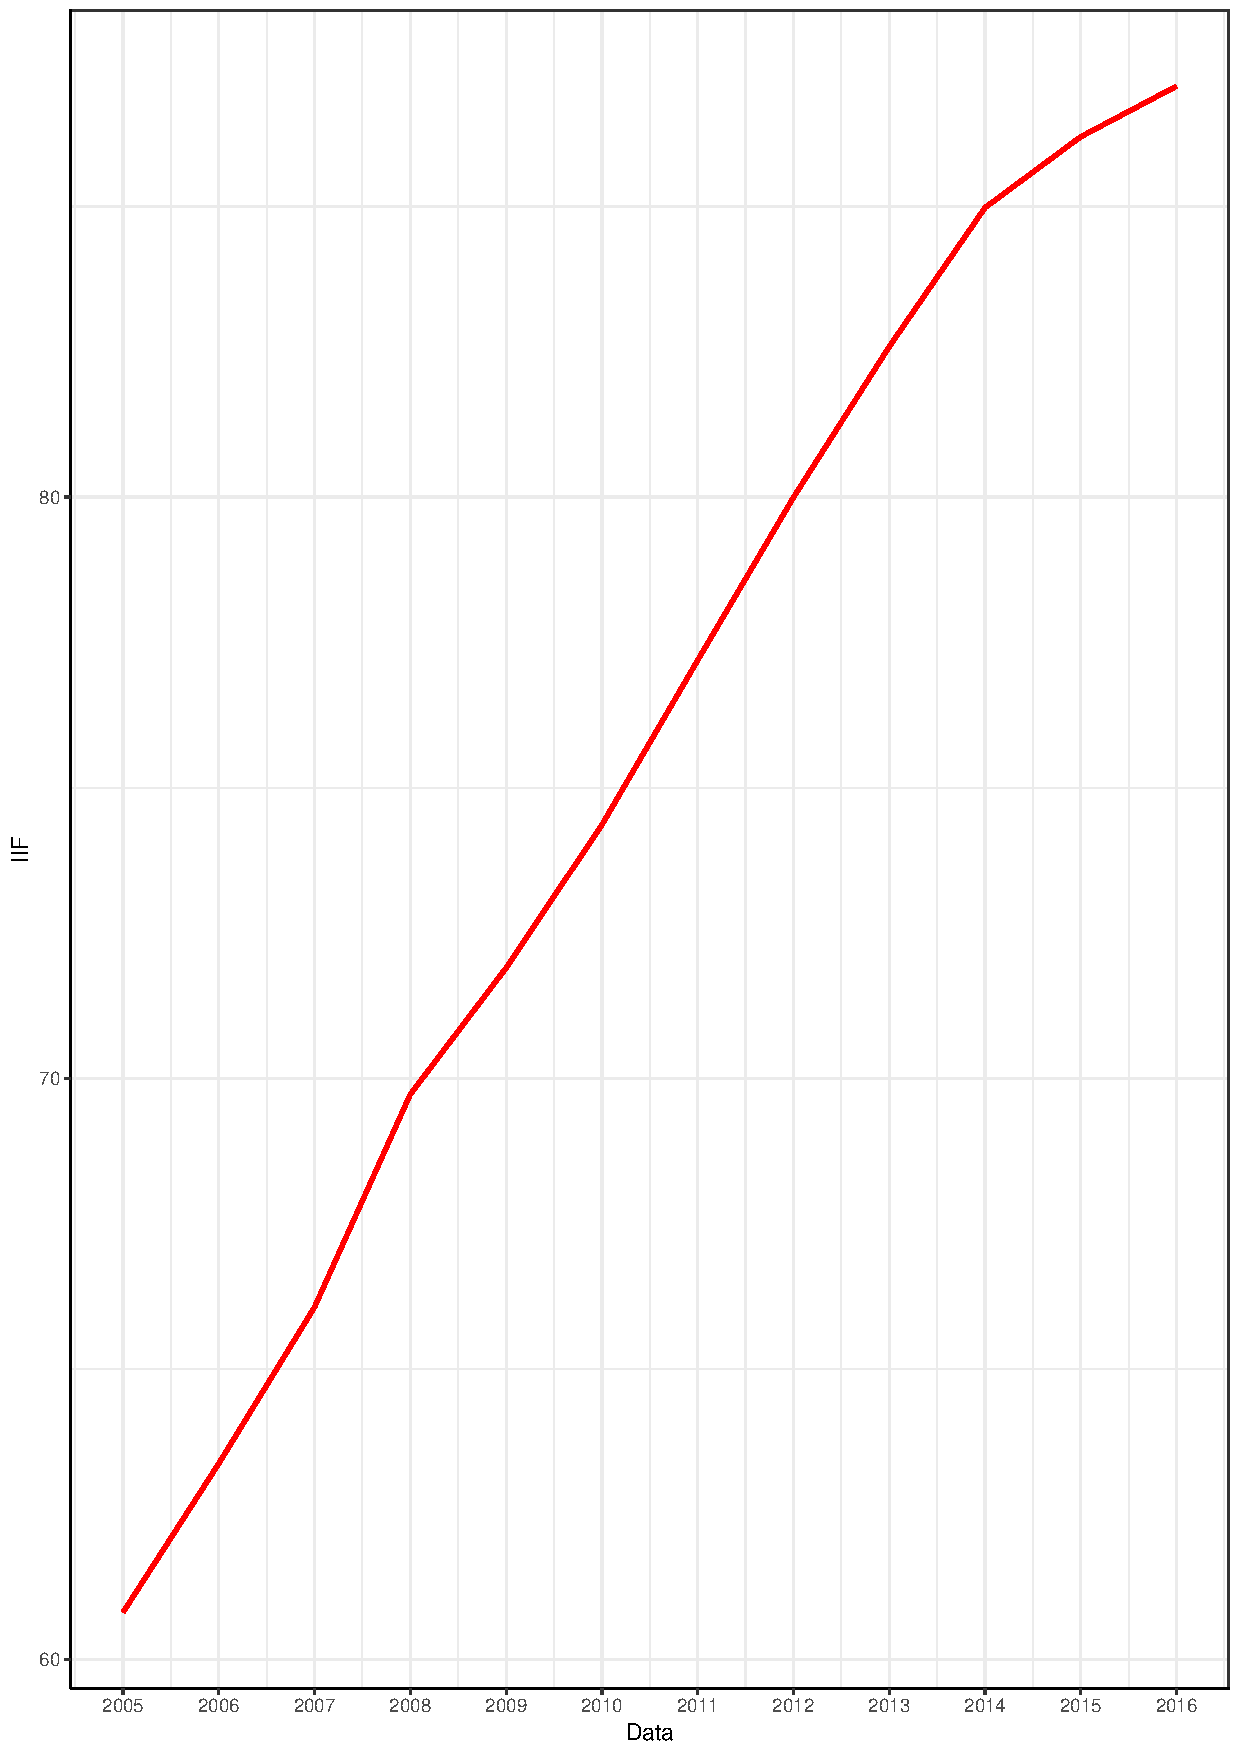
\includegraphics[width=0.8\paperwidth,height=0.8\paperheight]{plot.pdf}
\end{figure}
\end{frame}


\begin{frame}{Inclusão financeira}
\framesubtitle{Delimitando o conceito}
No entanto, a inclusão financeira não será aqui compreendida como um mero aprimoramento  institucional. Neste caso, será tratada como uma política deliberada de ampliação do sistema bancário na dinâmica econômica via expansão do crédito em extratos específicos da renda. Nesses termos, não é entendida como uma bancarização, mas sim como uma \textbf{desmarginalização creditícia}.
\end{frame}

\begin{frame}{Inclusão financeira}
\framesubtitle{Expansão do crédito}
\begin{figure}
	\centering
	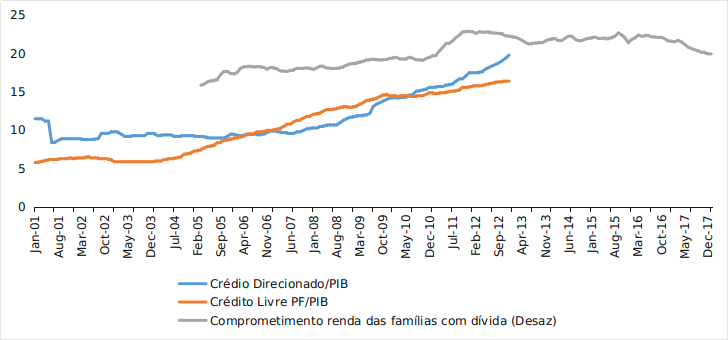
\includegraphics[width=1.2\textheight]{Credito.png}
\end{figure}
\end{frame}


\begin{frame}{Uma passo para trás...}
    Antes de prosseguir, é preciso evidenciar alguns pontos. Foram destacados dois elementos:
    \begin{itemize}
        \item Distribuição de renda (Estrutural)
        \item Inclusão financeira (Conjuntural)
    \end{itemize}
    A interpretação desse episódio requer a análise de outra esfera: \textbf{Institu\-cional}. Por ser de fundamental importância para a operacionalidade do Sistema Financeiro Nacional (SFN), o ambiente institucional a ser analisado é o Regime de Metas para a inflação.
\end{frame}

\begin{frame}{NCM e o Regime de metas para a inflação}
	Neste arcabouço:
	\begin{description}
		\item[Principal instrumento] Taxa de juros de curto prazo
		\item[Aparato institucional] Regime de Metas para a Inflação
		\item[Objetivo] Estabilização da inflação
	\end{description}
\begin{framed}



\begin{figure}[H]
	\centering
	\caption{Canal de transmissão}
	\label{ADFont}
	\vspace{-1cm}
	\[\Delta i \Rightarrow \Delta r \Rightarrow \Delta C \& \, \Delta I \Rightarrow \Delta AD \Rightarrow \Delta Y \& \, \Delta UN \Rightarrow \Delta (y - \overline{y}) \Rightarrow \Delta \pi\]
	\caption*{Fonte: \textcite[ p.~10]{Fontana}}
\end{figure}
\end{framed}
\end{frame}

\begin{frame}{Algumas críticas ao IT}
\textcite{Fontana} destaca alguns problemas do Regime de metas:
\begin{itemize}
	\item Viés de desemprego
	\item Efeitos distributivos
	\item Efeitos de instabilidade financeira
\end{itemize}
\vspace{1cm}
\begin{quotation}
	Os efeitos distributivos, por suas vez, decorrem de dois impactos da taxa de juros. O
	primeiro deles é o repasse dos custos financeiros para os preços. Isso ocorre porque, do ponto
	de vista das firmas, os juros são uma fonte de custo. Assim, sob uma estrutura de mercado
	oligopolizada, estes custos recairão sob os consumidores. O segundo impacto diz respeito à
	riqueza financeira. Isso decorre do fato que os juros são parâmetros de valorização da riqueza
	privada, favorecendo o setor rentista em detrimento do setor produtivo. \cite[p.~23]{Mono_Gabriel}
\end{quotation}
\end{frame}

\begin{frame}{Regima de Metas e Distribuição de renda}
Tanto o favorecimento do setor rentista quanto os efeitos negativos sobre a distribuição de renda são temas constantemente relatados na literatura. O que diferencia esta investigação das demais é a caracteriza\-ção desses efeitos em uma estrutura societária muito desigual em que houve uma crescente partipação do sistema bancário na dinâmica do consumo. Tendo em vista tais mudanças é que se pretende avialiar se houve ou não um conflito neste arranjo político-institucional-estrutural.
\end{frame}


\begin{frame}{Compatibilidade ou conflito?}
\framesubtitle{Trindade distributiva imposível?}
    \newcommand{\pythagwidth}{3cm}
\newcommand{\pythagheight}{3cm}
\begin{tikzpicture}
  \coordinate [label={below right:Inclusão financeira}] (A) at (0, 0);
  \coordinate [label={above:Distribuição de renda}] (B) at (-1.5, \pythagheight);
  \coordinate [label={below left:Regime de Metas}] (C) at (-\pythagwidth, 0);

  \coordinate (D1) at (-\pythagheight, \pythagheight + \pythagwidth);
  \coordinate (D2) at (-\pythagheight - \pythagwidth, \pythagwidth);

  \draw [very thick] (A) -- (C) -- (B) -- (A);


  \end{tikzpicture}
\end{frame}

\begin{frame}{Conclusão Preliminar}
    A principal hipótese levantada desse estudo é que este \textbf{arranjo} gerou uma relação conflituosa entre os objetivos de política econômica, os instrumentos utilizados e o ambiente institucional. No entanto, essa conclusão não implica em impossibilidade de distribuição de renda a favor dos salários, mas sim de que tal objetivo deve ser perseguido de outra maneira:
    \begin{itemize}
        \item Reformulação do regime de metas para se adequar à especificidade do Brasil: elevada desigualdade
        \item Distribuição de renda ser feita à partir de mudanças na estrutura, dificultando sua reversão e diminuindo a endogeinização de seus limites
    \end{itemize}
\end{frame}

\begin{frame}
\frametitle{Dados}
\framesubtitle{Distribuição de renda}
    \begin{itemize}
        \item Índice de Theil-L
        \item Percentis
            \begin{itemize}
                \item 10\% em relação aos 40%
                \item 50\%, 40\%, 10\% e 1\%
            \end{itemize}
        \item Base de dados WID
        \item World Bank (Comparação internacional)
    \end{itemize}
\end{frame}


\begin{frame}
\frametitle{Dados}
\framesubtitle{Inclusão financeira}
    \begin{itemize}
        \item Índice de inclusão financeira global (IFI - \textit{Global Index})
        \item Séries temporais do BCB
        \begin{itemize}
            \item Adultos com relacionamento bancário por região, faixa etária
            \item Clientes detentores de contas por faixa de depósito de poupança
            \item Saldo de consórcio
            \item SCFIs
            \item Crédito livre e direcionado à Pessoa Física
            \item Comprometimento da renda das famílias com dívida
        \end{itemize}
        \item Outras séries relacionadas
    \end{itemize}
\end{frame}

\begin{frame}{Bibliografia}
    O material consultado será dividido em três categorias para cada um dos itens a serem analisados:
    \begin{itemize}
        \item Literatura teórica
        \item Análise comparativa internacional
        \item Debate para o caso brasileiro
    \end{itemize}
    Estas categorias bibliográficas tem como objetivo orientar e contextuali\-zar o tema proposto assim como anteceder a análise dos dados especificados anteriormente
\end{frame}


\begin{frame}{Questões em aberto}
    Esta apresentação tentou explicitar o caminho a ser traçado por esta pesquisa sem, no entanto, utilizar uma metodologia própria e única. A princípio, estuda-se a possibilidade de utilizar a metodologia \textit{Agent Based}. 
    
    \begin{description}
    \item[Vantagem] É uma metodologia que se ajusta bem em situações em que a heterogeneidade dos agentes econômicos importa além de ser uma contribuição para esta fronteira de pesquisa
    \item[Desvantagem] Além da dificuldade operacional de se construir tal modelo, há a desvantagem de ser uma abordagem ainda em construção e muitos instrumentos necessários podem ser mais difícies de serem utilizados
    \end{description}
\end{frame}

\begin{frame}{Possíveis críticas e respostas}
    O presente estudo tem limitações evidentes que, apesar de não invalidarem os argumentos apresentados, devem ser analisadas e tentarão ser contarnadas ao longo da pesquisa:
    \begin{itemize}
        \item Abordagem fica muito restrita à política econômica e pouco diz sobre a economia política
            \begin{description}
            \item[Resposta:] Tais fatores serão evidenciados em um capítulo a parte (Introdução e/ou conclusão)
            \end{description}
        \item Regime de Metas não é o único (e talvez mais importante) elemento institucional
             \begin{description}
            \item[Resposta:] A presente abordagem não nega a importância das demais, apenas evidencia a incompatibilidade gerada pelo arranjo
            \end{description}
       
    \end{itemize}
\end{frame}

\begin{frame}{Possíveis críticas e respostas (continuação)}
\begin{itemize}
 \item Distribuição funcional da renda em favor dos salários requer aumento na produtividade
            \begin{description}
            \item[Resposta:] Tal hipótese precisa ser analisada, mas foge do escopo deste trabalho
            \end{description}
        \item E o setor externo e a GFC?
            \begin{description}
            \item[Resposta:] Tais perturbações serão analisadas, mesmo que com menor detalhe, na medida que os dados forem apresentados
            \end{description}
\end{itemize}
\end{frame}

\begin{frame}{Para onde estamos indo?}
\newcommand{\pythagwidth}{3cm}
\newcommand{\pythagheight}{3cm}
\begin{tikzpicture}
  \coordinate [label={below right:Inclusão financeira}] (A) at (0, 0);
  \coordinate [label={above:\sout{Distribuição de renda}}] (B) at (-1.5, \pythagheight);
  \coordinate [label={below left:Regime de Metas}] (C) at (-\pythagwidth, 0);

  \coordinate (D1) at (-\pythagheight, \pythagheight + \pythagwidth);
  \coordinate (D2) at (-\pythagheight - \pythagwidth, \pythagwidth);

  \draw [very thick] (A) -- (C) -- (B) -- (A);


  \end{tikzpicture}
    
\end{frame}


\frame[allowframebreaks]{  \frametitle{Referências bibliográficas}
\framesubtitle{Em construção}


\printbibliography
}





\end{document}